\newpage

\section{Matching}
\subsection{Bipartite matching}
\begin{figure}[H]
    \centering
    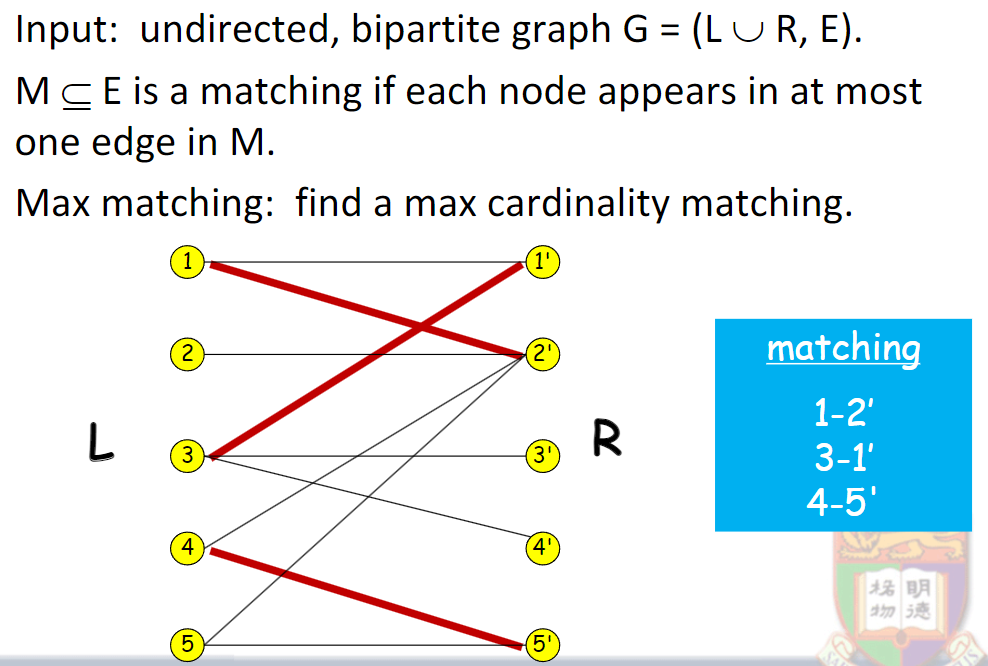
\includegraphics[width=0.309\textwidth]{pic/DAA10/Bipartite matching}
    \caption{Bipartite matching}
\end{figure}

\subsubsection{Bipartite Matching and Max Flow}
\begin{figure}[H]
    \centering
    \begin{subfigure}{0.309\textwidth}
        \centering
        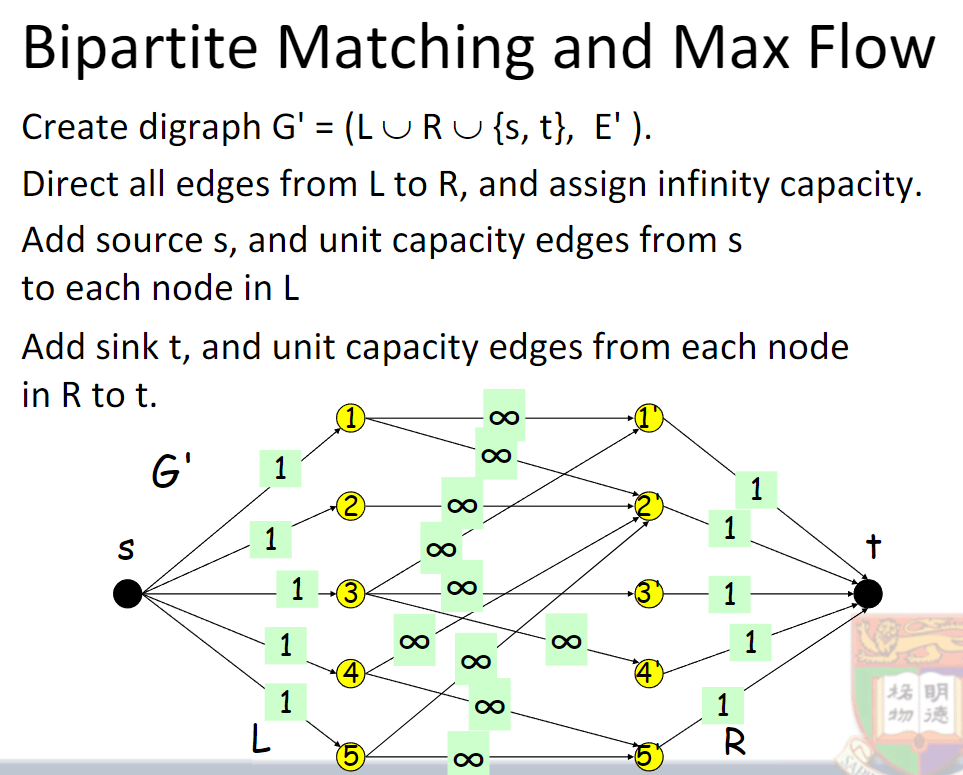
\includegraphics[width=\textwidth]{pic/DAA10/Bipartite matching and Max Flow}
    \end{subfigure}
    \begin{subfigure}{0.309\textwidth}
        \centering
        \includegraphics[width=\textwidth]{pic/DAA10/Bipartite matching and Max Flow2}
    \end{subfigure}
    \caption{Bipartite matching and Max Flow}
\end{figure}

\subsubsection{Alternating Path Approach}
\begin{figure}[H]
    \centering
    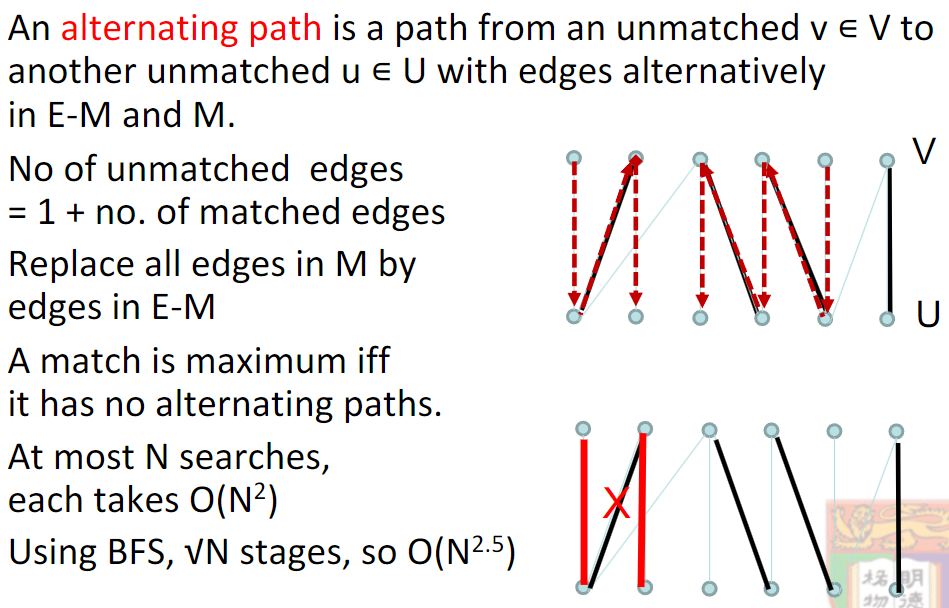
\includegraphics[width=0.309\textwidth]{pic/DAA10/Alternating Path Approach}
    \caption{Alternating Path Approach}
\end{figure}


\subsection{Perfect Matching}
\begin{figure}[H]
    \centering
    \begin{subfigure}{0.309\textwidth}
        \centering
        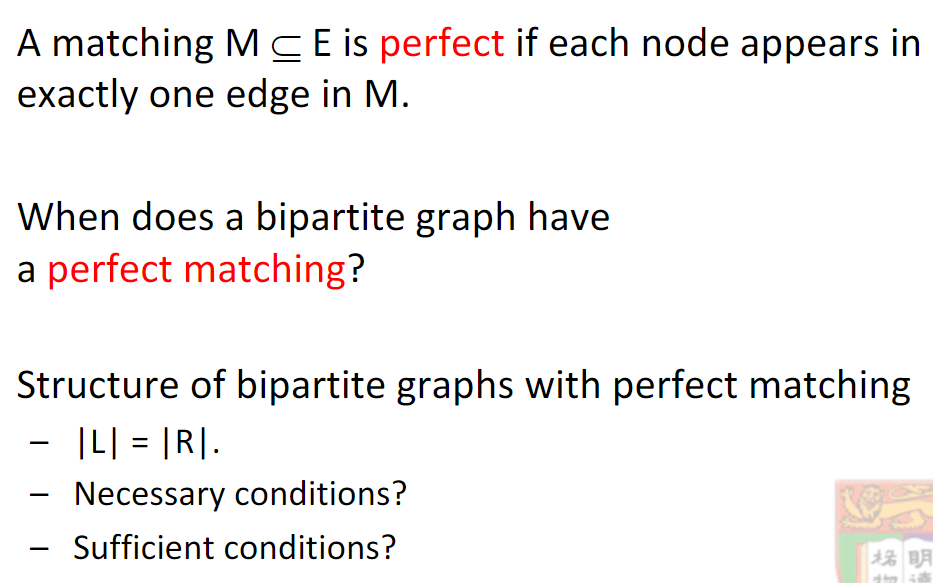
\includegraphics[width=\textwidth]{pic/DAA10/Perfect Matching1}
    \end{subfigure}
    \begin{subfigure}{0.309\textwidth}
        \centering
        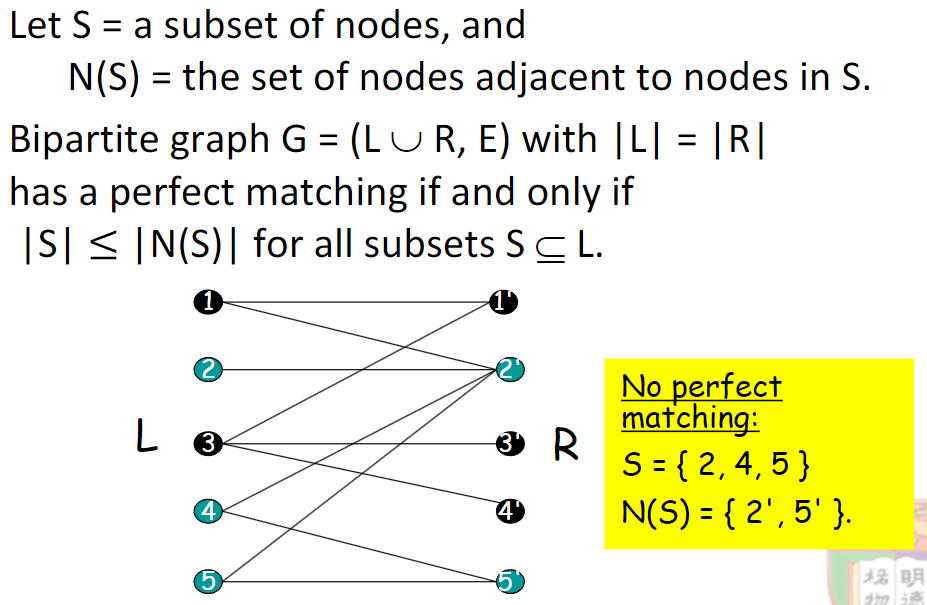
\includegraphics[width=\textwidth]{pic/DAA10/Perfect Matching2}
    \end{subfigure}
    \caption{Perfect Matching}
\end{figure}

\subsubsection{Marriage Theorem}
\begin{figure}[H]
    \centering
    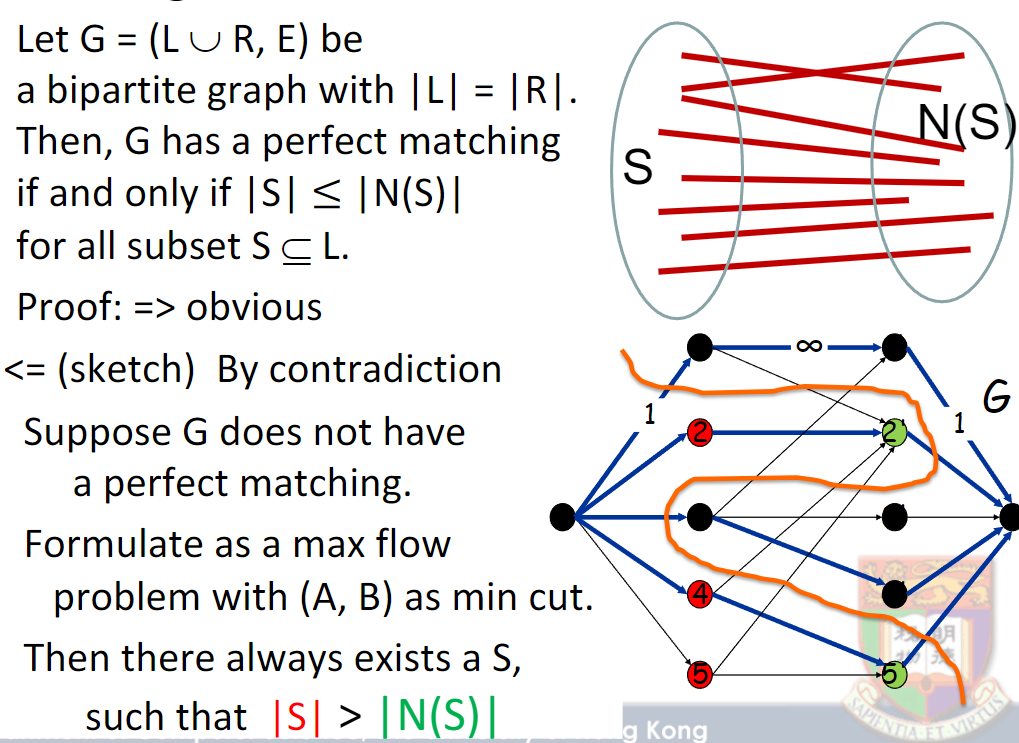
\includegraphics[width=0.309\textwidth]{pic/DAA10/Marriage Theorem}
    \caption{Marriage Theorem}
\end{figure}


\subsection{Perfect Matching for Dense Graph}



\subsection{Stable Marriage}
\begin{figure}[H]
    \centering
    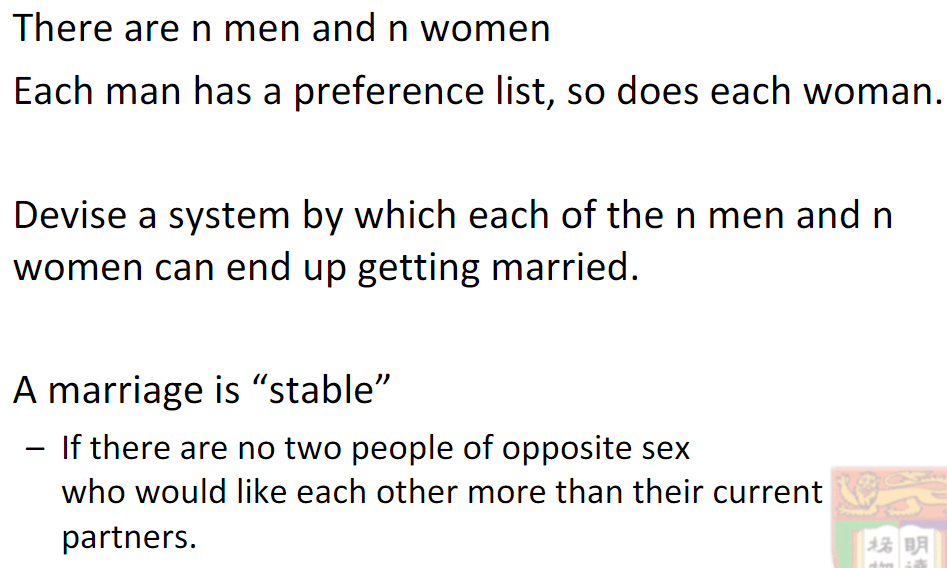
\includegraphics[width=0.309\textwidth]{pic/DAA10/Stable Marriage}
    \caption{Stable Marriage}
\end{figure}

\subsubsection{Example Preference Lists}
\begin{figure}[H]
    \centering
    \begin{subfigure}{0.309\textwidth}
        \centering
        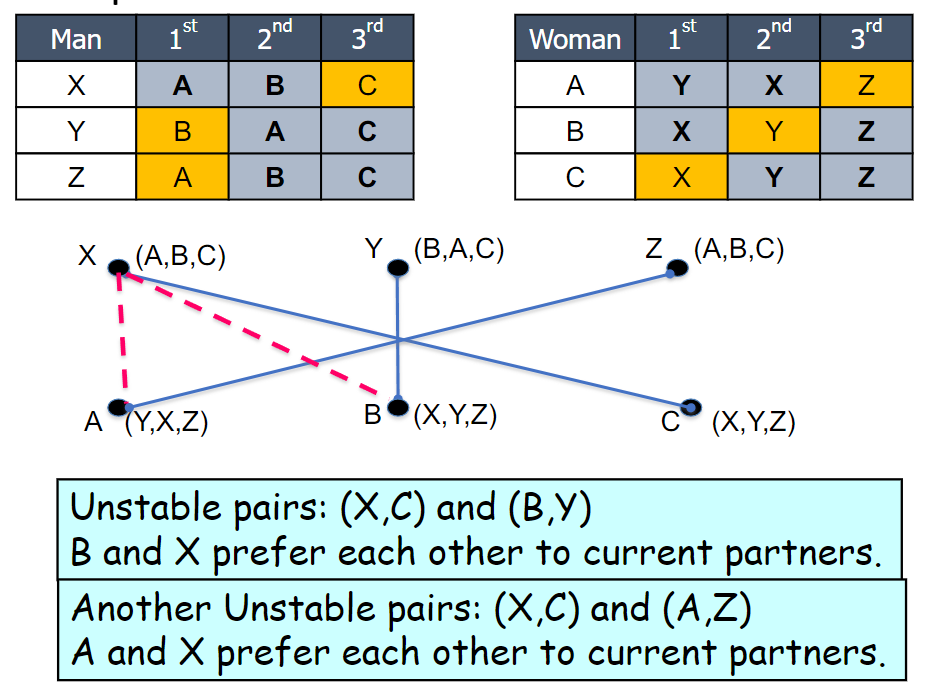
\includegraphics[width=\textwidth]{pic/DAA10/Example Preference Lists1}
    \end{subfigure}
    \begin{subfigure}{0.309\textwidth}
        \centering
        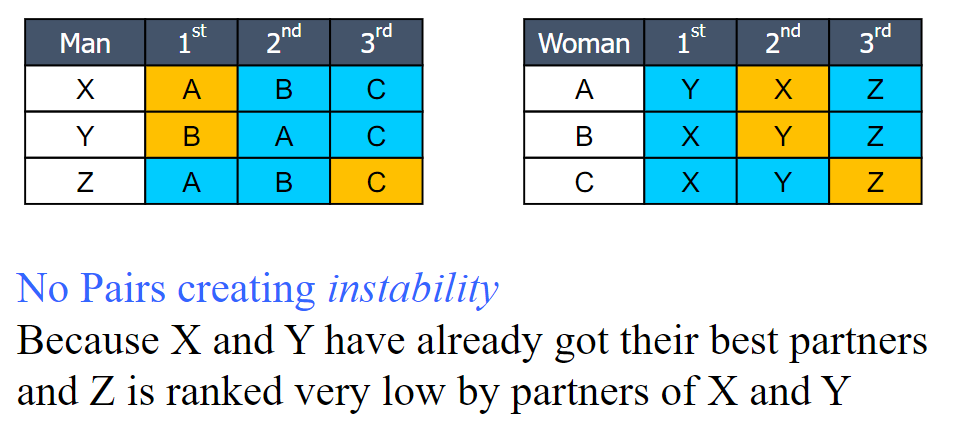
\includegraphics[width=\textwidth]{pic/DAA10/Example Preference Lists2}
    \end{subfigure}
    \caption{Example Preference Lists}
\end{figure}

\subsubsection{Gale-Shapley (GS) Algorithm}
Men Propose (Women dispose)
\begin{figure}[H]
    \centering
    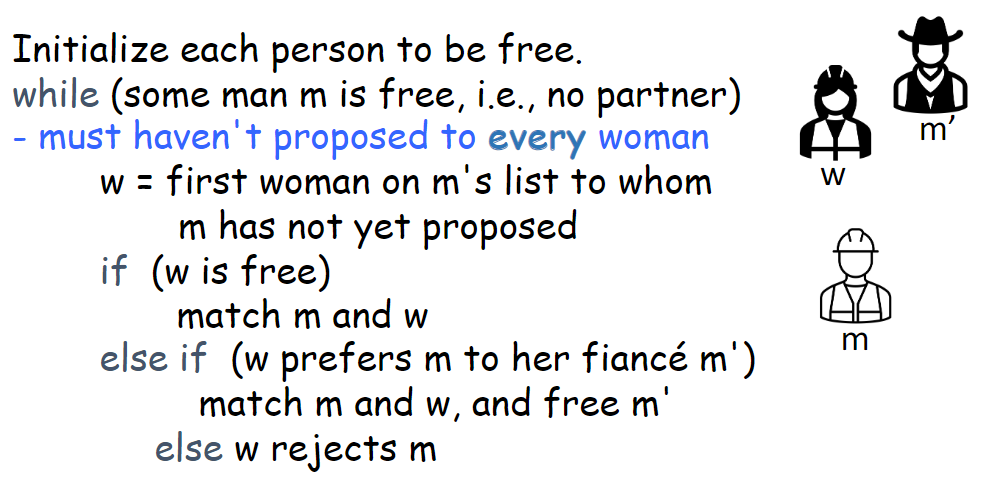
\includegraphics[width=0.309\textwidth]{pic/DAA10/Gale-Shapley (GS) Algorithm}
    \caption{Gale-Shapley (GS) Algorithm}
\end{figure}

后面是对这个算法的分析, 摸了.

不对, 我感觉这个肯定要考, 看看.

\begin{figure}[!htb]
    \centering
    \begin{subfigure}{0.309\textwidth}
        \centering
        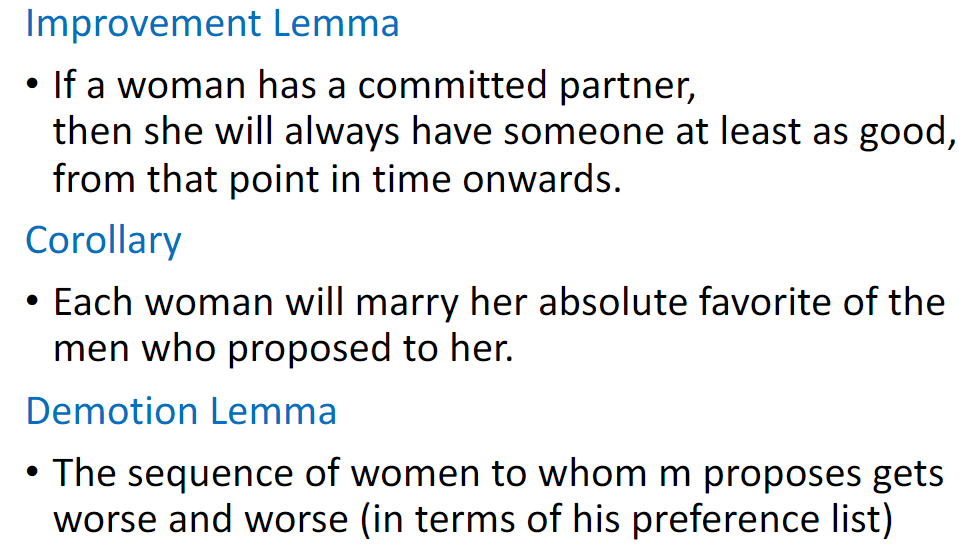
\includegraphics[width=\textwidth]{pic/DAA10/Facts}
    \end{subfigure}
    \begin{subfigure}{0.309\textwidth}
        \centering
        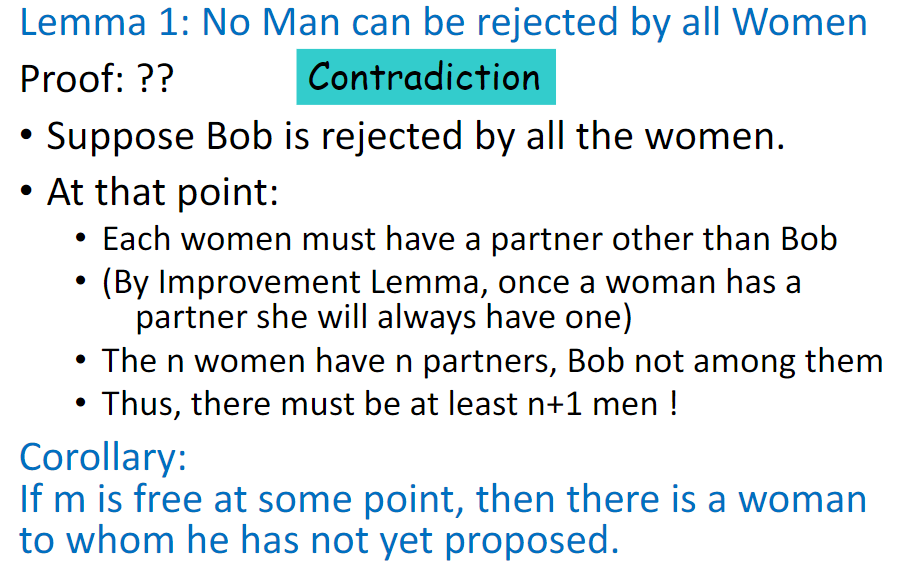
\includegraphics[width=\textwidth]{pic/DAA10/Facts1}
    \end{subfigure}
    \begin{subfigure}{0.309\textwidth}
        \centering
        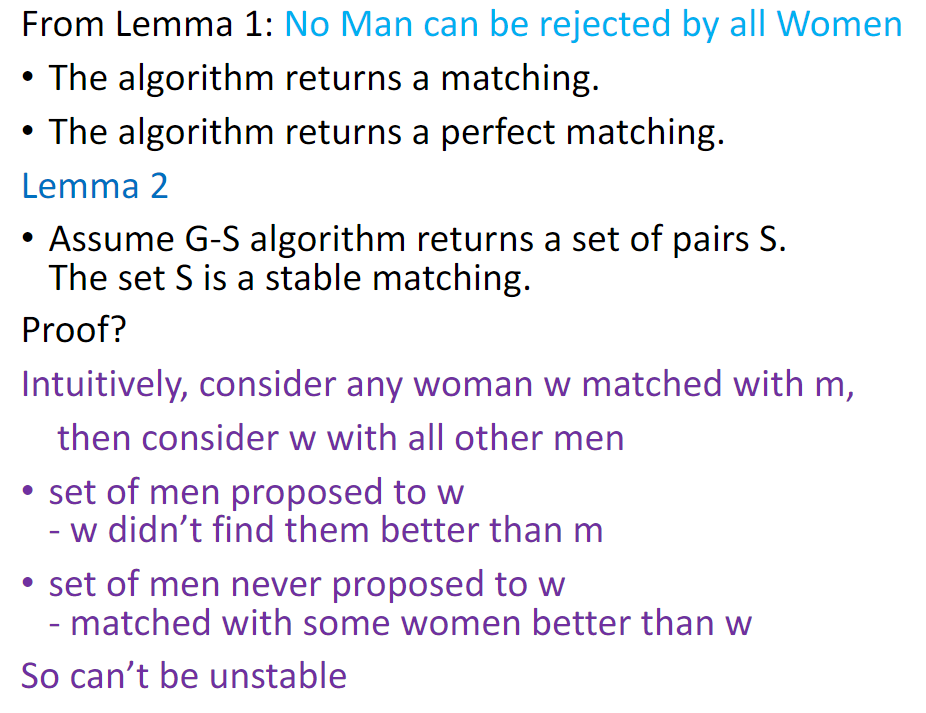
\includegraphics[width=\textwidth]{pic/DAA10/Facts2}
    \end{subfigure}
    \begin{subfigure}{0.309\textwidth}
        \centering
        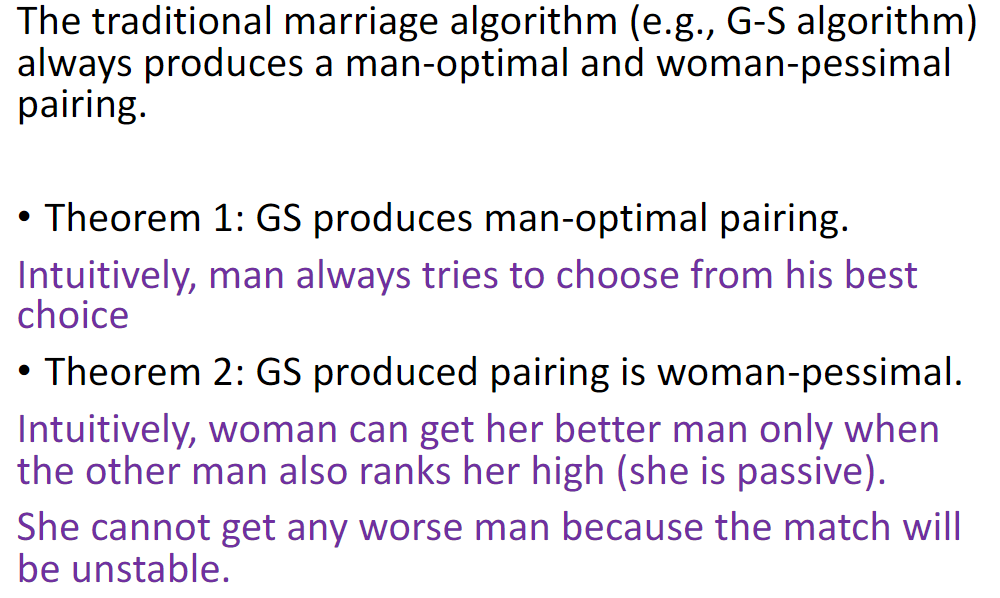
\includegraphics[width=\textwidth]{pic/DAA10/Facts3}
    \end{subfigure}
    \caption{Facts}
\end{figure}



\subsection{Assignment Problem}
